\section{Temperature and chlorophyll response to ENSO variability}
\label{sec:pisces}

The ocean fish biomass is strongly influenced by the physical and biogeochemical state of the ocean. Therefore, it is important to determine whether the NEMO-PISCES model, which is used to force the Apecosm model, accurately reproduces the expected response to ENSO variability. Although successfully used in a variety of ENSO-related physical and biogeochemical studies in the tropical Pacific (e.g., Vialard et al. 2001, Lengaigne et al. 2002; Lengaigne et al., 2007; Schneider et al., 2008; Masotti et al. 2011; Currie et al. 2013), the ability of our simulation to capture ENSO surface temperature and chlorophyll signature satellite surface Chl is briefly evaluated in the present section.

ENSO variability is characterized here by the well-known Ocean Niño Index (ONI). The ONI index simulated by the model compares very well with the observed one (Fig. 1??), with correlation coefficient between the two time-series reaching 0.94 over their common 1958-2018 period. In particular, the model is able to accurately capture the timing and amplitude of major El Niño events, like in 1972/73, 1982/83, 1997/98 and 2015/16 and of major La Niña events, like in 1988/89 and 1999/2000 . The ENSO SST pattern is evaluated  by calculating the covariance between the ONI and detrended SST anomalies over the tropical Pacific in boreal winter (November to January), i.e. when ENSO variability is the largest. The ONI index has been averaged over boreal winter (from November to January), when most of  the ENSO variability occurs. In order to ensure continuity over the winter months, when ENSO variability usually peaks, yearly means of SST have been computed from May (year y) to April (year y + 1), as done in (Racault et al., 2017). Then, the obtained time-series has been detrended. The covariance between the ONI index and the sea-surface temperature is shown in Figure 1. The same operation has been repeated with the simulated SST (bottom panel).

Modelled ENSO SST  pattern closely resembles  the observed one. This pattern is characterized by warm SST anomalies (1\degree{}C) centred in the central and eastern equatorial Paciic  flanked by the traditional horseshoe cooling pattern in the western Pacific extending towards the subtropical north and south Pacific. This SST seesaw in the equatorial region is further accompanied by a shoaling of the thermocline in the west and a deepening in the east (not shown).

\begin{figure}[h!]
	\centering
	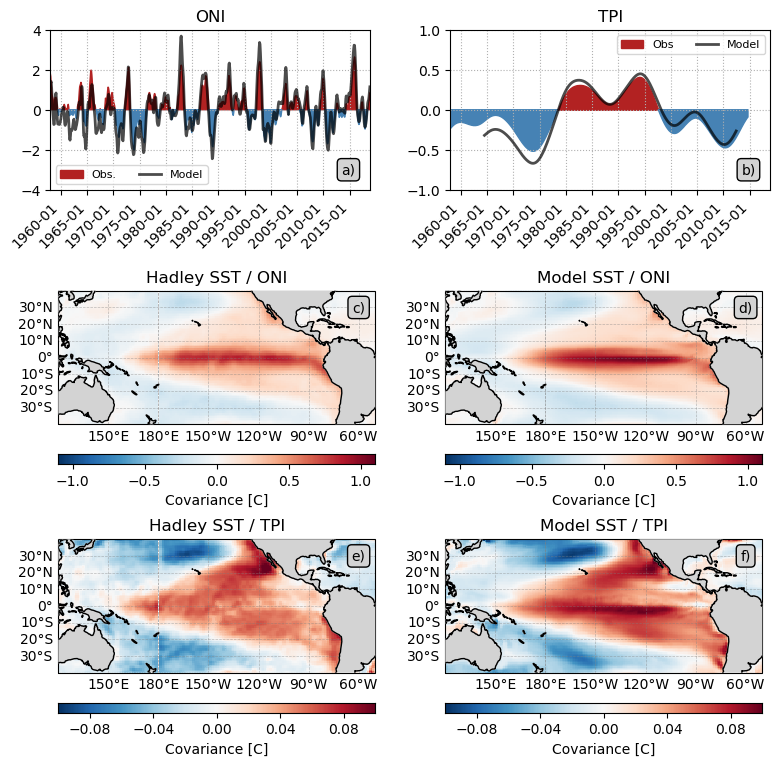
\includegraphics[scale=0.75] {scripts/final_figs/fig1/fig1.png}
	\label{fig:cov-sst}
\end{figure}

\begin{figure}[h!]
	\centering
	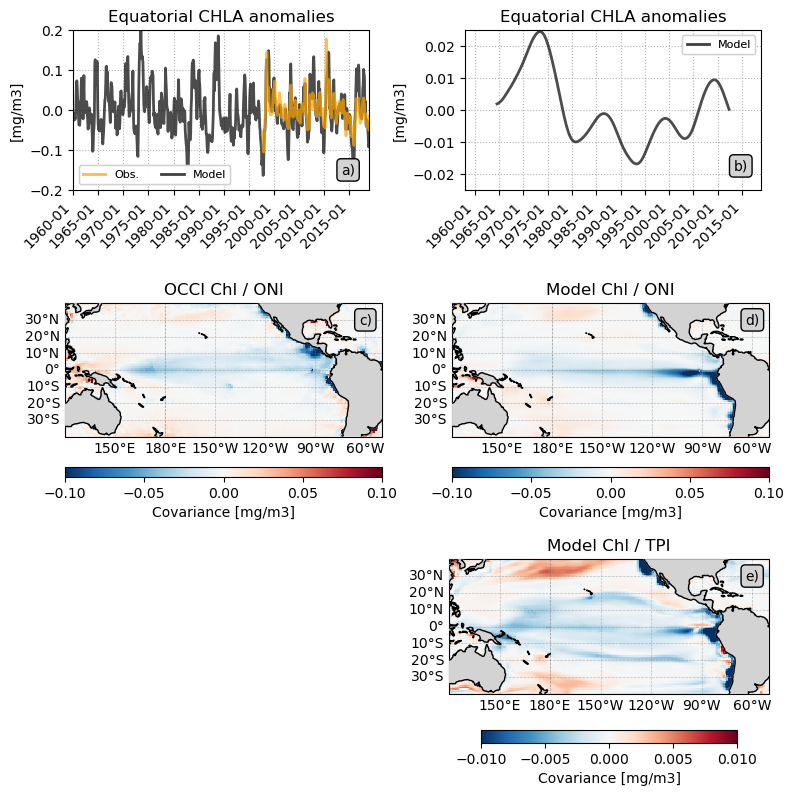
\includegraphics[scale=0.75] {scripts/final_figs/fig2/fig2.png}
	\label{fig:cov-chl}
\end{figure}

Covariance maps between the surface chlorophyll and the monthly ONI index are shown in Fig 1. The observations (upper panel) and the model (lower panel) show very similar covariance pattern: El Niño induces a decrease in chlorophyll concentration in the along the equator east of 150\degree{}E, consistent with a weaker equatorial upwelling induced by the equaotiral trade winds reduction. However, the model overestimates the chlorophyll response to ENSO variability compared with observational based estimates. Note that the covariance for the simulated chlorophyll has also been computed over the entire simulated period (1958-2018), with no significant changes in the resulting pattern (not shown).